%%%%%%%%%%%%%%%%%%%%%%%%%%%%%%%%%%%%%%%
%%%  ISWC 2018 - NERD for NexGenTv  %%%
%%%%%%%%%%%%%%%%%%%%%%%%%%%%%%%%%%%%%%%

\documentclass{llncs}

\usepackage{graphicx}
\usepackage{xtab}
\usepackage{xfrac}
% explicitly commented
% \usepackage[table,xcdraw]{xcolor}
\usepackage{amsmath}
\usepackage{amssymb}
\usepackage[inline]{enumitem}
% \usepackage[capposition=top]{floatrow}
\usepackage{pifont}
\usepackage{cite}
\newcommand{\cmark}{\ding{51}}
\newcommand{\xmark}{\ding{55}}
\DeclareGraphicsExtensions{.png}

\newenvironment{conditions*}
  {\par\vspace{\abovedisplayskip}\noindent
   \tabularx{\columnwidth}{>{$}l<{$} @{\ : } >{\raggedright\arraybackslash}X}}
  {\endtabularx\par\vspace{\belowdisplayskip}}
  
\newcommand{\secref}[1]{\mbox{Section~\ref{#1}}}
\newcommand{\tabref}[1]{\mbox{Table~\ref{#1}}}
\newcommand{\figref}[1]{\mbox{Figure~\ref{#1}}}
\newcommand{\eqnref}[1]{\mbox{Eqn~(\ref{#1})}}

\usepackage{todonotes}

\graphicspath{ {images/} }
%% Save the class definition of \subparagraph
\let\llncssubparagraph\subparagraph
%% Provide a definition to \subparagraph to keep titlesec happy
\let\subparagraph\paragraph
\usepackage{titlesec}
\usepackage{hyperref}
%% Revert \subparagraph to the llncs definition
\let\subparagraph\llncssubparagraph

\titleformat{\subsection}[runin]{\bfseries}{}{}{}[]

%%%%%%%%%%%%%%%%%%%%%%%%%%%%%%%
%%%  Beginning of document  %%%
%%%%%%%%%%%%%%%%%%%%%%%%%%%%%%%

\begin{document}

\title{A Novel Ensemble Method for Named Entity Recognition and Disambiguation based on Neural Network}

\author{
Lorenzo Canale\inst{1,2} \and Pasquale Lisena\inst{1}
\and Rapha\"el Troncy\inst{1}}
\authorrunning{Canale et al.}
\institute{EURECOM, Sophia Antipolis, France \\
\email{\{canale|lisena|troncy\}@eurecom.fr} \and 
Politecnico di Torino, Italy 
% \email{lorenzo.canale@studenti.polito.it}
}

\maketitle

%%%%%%%%%%%%%%%%%%
%%%  Abstract  %%%
%%%%%%%%%%%%%%%%%%

\begin{abstract}
Named entity recognition (NER) and disambiguation (NED) are subtasks of information extraction that respectively aim to recognize named entities mentioned in text, to assign them pre-defined types, and to link them with their matching entities in a knowledge base. Many approaches, often exposed as web APIs, have been proposed to solve these tasks during the last years. These APIs classify entities using different taxonomies and disambiguate them with different knowledge bases. In this paper, we describe Ensemble Nerd, a framework that collects numerous extractors responses, normalizes them and combines them in order to produce a final entity list according to the pattern (surface form, type, link). The presented approach is based on representing the extractors responses as real-value vectors and on using them as input samples for two Deep Learning networks: ENNTR (Ensemble Neural Network for Type Recognition) and ENND (Ensemble Neural Network for Disambiguation). We train these networks using specific gold standards. We show that the models produced outperform each single extractor responses in terms of micro and macro F1 measures computed by the GERBIL framework. 
\end{abstract}

%%%%%%%%%%%%%%%%%%%%%%%%
%%% 1. Introduction  %%%
%%%%%%%%%%%%%%%%%%%%%%%%

\section{Introduction}
\label{sec:introduction}
A crucial task in knowledge extraction from textual document consists in the two complementary tasks of Named Entity Recognition (NER) and Named Entity Disambiguation (NED), achieving the goal of assigning to parts of text (tokens) respectively a type -- from a pre-defined taxonomy -- and an unique identifier -- normally in the form of URI -- that points univocally to the referred entity in a given knowledge base. The combination of these two tasks is often abbreviated with the acronym NERD~\cite{nerd1,nerd2}. The current state of the art offers an interesting number of NERD extractors. Some of them can be trained by a developer on his own corpus, while other ones are only accessible as black-box services exposed via web APIs offering a limited number of parameters.

In terms of NER, each service provides generally its own taxonomy of named entity types which can be recognised. While they all provide support for three major types (person, organization, location), they largely differ for more fine-grained types which makes hard their comparison and combination. In terms of NED, each extractor can potentially disambiguate entities against specific knowledge bases (KB), but in practice, they mostly rely on popular ones, namely DBpedia, Wikidata, Freebase or YAGO. For this reason, comparing and merging the results of these extractors require some post-processing tasks that typically rely on mappings between those KBs. This task is however simpler than the type alignment, because of the large presence of interlinks between the different KBs.

In this paper, we present \textbf{Ensemble Nerd}, a multilingual ensemble method that combines the responses of different NERD extractors. This method relies on a real-value vectorial representation as input samples for two Deep Learning networks, ENNTR (Ensemble Neural Network for Type Recognition) and ENND (Ensemble Neural Network for Disambiguation). The networks provide as output models for performing type alignment and named entity linking to the DBpedia, Wikipedia and Wikidata knowledge bases. This strategy is evaluated against some well-known gold standards, showing that the output of the ensemble outperforms the results of single extractors. 

This work aims to answer the following research questions: Can we define an ensemble method that combines the extractors responses in order to create a new more powerful extractor? Is it possible to define an ensemble method that avoids a type alignment step or that computes it automatically, without any human intervention? Which ensemble method should be adopted to exploit all the collected information? Considering that extractors return list of named entities -- together with the type and the disambiguation link of each of them --, how this data can be numerically represented? Can we better understand which features contribute more to improve the ensemble output response? How dependant is this feature selection of the corpora, language, entity types and what is the influence of the KB?

The remainder of this paper is organized as follows. In \secref{sec:state-of-art}, we describe some related work. In \secref{sec:study}, we detail how we represent the extractors responses, while in \secref{sec:experiment}, we present the core of our ensemble method. We propose an evaluation in the \secref{sec:evaluation}. Finally, we summarize our main findings and outline some future work in Section \secref{sec:conclusion}.

%%%%%%%%%%%%%%%%%%%%%%%%%%%%
%%% 2. State of the art  %%%
%%%%%%%%%%%%%%%%%%%%%%%%%%%%

\section{State of the Art}
\label{sec:state-of-art}
Ensemble methods in NER and NED tasks have been largely studied with different approaches.

The \textbf{NERD} framework~\cite{nerd1,nerd2} allows to compare and evaluate some of the most popular Linked Data named entity extractors.
It is able to analyse any textual resource published on the web and to extract the named entities that are detected, typed and disambiguated by various named entity extractor APIs. For overcoming the different type taxonomies, the authors designed the \textit{NERD ontology} which provides a set of mappings between these various classifications and consequently makes possible an evaluation of the quality of each extractor. This task was originally a one time modeling exercise: the authors manually mapped the different taxonomies to the NERD ontology.
However in \cite{nerd4}, they proposed a more sophisticated and robust approach that uses machine learning inductive techniques for passing from the output type of single extractors to the right entity type in a normalized types set, i.e. the NERD Ontology. The used algorithms are alternatively k-Nearest Neighbour (k-NN) and Naive Bayes (NB).

\textbf{NERD-ML}, a machine learning approach developed on top of the NERD framework, combines the responses of single extractors applying alternatively three different  algorithms: Naive Bayes (NB), k-Nearest Neighbours (k-NN) and Support Vector Machines (SVM)~\cite{nerd2,nerd3}. \textbf{FOX}~\cite{fox1,fox2} is a framework that relies on ensemble learning by integrating and merging the results of four NER tools: the \textbf{Stanford Named Entity Recognizer}~\cite{Finkel:2005:INI:1219840.1219885},
the \textbf{Illinois Named Entity Tagger}~\cite{Ratinov:2009:DCM:1596374.1596399},
the \textbf{Ottawa Baseline Information Extraction} (Balie) and the \textbf{Apache OpenNLP Name Finder}. FOX compares the performance of these tools for a small set of classes namely LOCATION, ORGANIZATION and PERSON. For achieving this goal, the entity types of each NER tools is mapped to these three classes. Given any input text $t$, FOX processes $t$ with each of the $n$ tools it integrates. The result of each tool $T_i$ is a piece of annotated text $t_i$, in which either a specific class or zero (not belonging to the label of a named entity) is assigned to each token. The tokens in $t$ are then represented as vectors of length $n$ and are used for getting the final type. The author demonstrates that a Multi-Layer Perceptron (MLP) gets the best results among a pool of 15 different algorithms~\cite{fox2}.

%%%%%%%%%%%%%%%%%%%%%%%%%%%%%%%%%%%%%%
%%%  Feature Engineering for NERD  %%%
%%%%%%%%%%%%%%%%%%%%%%%%%%%%%%%%%%%%%%

\section{Feature Engineering for NERD}
\label{sec:study}
Ensemble Nerd currently integrates a set of 8 extractors showed in \tabref{tab:exout}. An extractor can belong to the set $T$ (extractors that perform NER task) or to the set $U$ (extractors that perform NED task). Currently, \textit{TextRazor} is the only one in both sets: $T \cap U = \left \{  TextRazor \right \}$. All these extractors relies on Wikidata, Wikipedia or DBpedia for entity disambiguation.
 
\begin{table}
\centering
\label{tab:exout}
\begin{tabular}{|c|c|c|}
\hline
\textbf{Extractor} & \textbf{Type recognition} & \textbf{NE disambiguation} \\ \hline
AlchemyAPI    & \cmark  & \xmark \\ \hline
DandelionAPI  & \xmark  & \cmark \\ \hline
DbSpotlight   & \xmark  & \cmark \\ \hline
TextRazor     & \cmark  & \cmark \\ \hline
Babelfy       & \xmark  & \cmark \\ \hline
MeaningCloud  & \cmark  & \xmark \\ \hline
Adel          & \cmark  & \xmark \\ \hline
OpenCalais    & \cmark  & \xmark \\ \hline
\end{tabular}
\bigskip
\caption{Extractor included in Ensemble Nerd. \cmark{ }indicates that the extractor supports the action (type recognition or named entity disambiguation)}.
\end{table}

Each extractor produces a list of named entities as response for a specific input text. From this output, we generate 4 different kinds of feature: surface form features, type features, entity features, score features.

\textbf{Surface form features}. They are strictly related to the text used to extract named entity. The input text is split into tokens and a word embedding representation is assigned to each of them. We consider as tokens also the stop words.
The word vectors are computed using \textit{fastText}~\cite{fasttext}. We define $\vec{s^{n}}$ as the real-valued vector associated to a specific token $n$:

\begin{equation}
\vec{s^{n}} = \left [  \vec{s^{n}_p}|\vec{s^{n}_c} \right ], dim(\vec{s^{n}})=400
\end{equation}
where: 
\begin{itemize}
    \item[] $|$ is the concatenation operator
    \item[] $dim$ is the dimension of the vector
\end{itemize}

$\vec{s^{n}_p}$, $dim(\vec{s^{n}_p})=300$, consists in the token embedding computed using the Wikipedia pre-trained \textit{fastText} models released by the authors. The model changes depending on the language used in the text, since all localised Wikipedia have been used to train language specific models.

$\vec{s^{n}_c}$, $dim(\vec{s^{n}_c})=100$, is the token embedding computed when training \textit{fastText} directly on a particular textual corpus -- i.e. the one for which we want to perform the NERD tasks. This means that $\vec{s^{n}_c}$ does not vary depending on the language but on the gold standard itself.

\textbf{Type features}. Each extractor $e \in T$ has its own type taxonomy $o$ which is a taxonomy of a maximum depth $L$. In the following, we consider a simple example of an taxonomy $o$ with just a 2 levels hierarchy (\figref{fig:ontology}):
\begin{enumerate}
\begin{item}
Level 1 includes three types: PLACE, ORGANIZATION and PERSON.
\end{item}
\begin{item}
Level 2 includes four types: CITY and MOUNTAIN (subtypes of PLACE) and ACTOR and MUSICIAN (subtypes of PERSON). 
\end{item}
\end{enumerate}

\begin{figure}
	\centering
    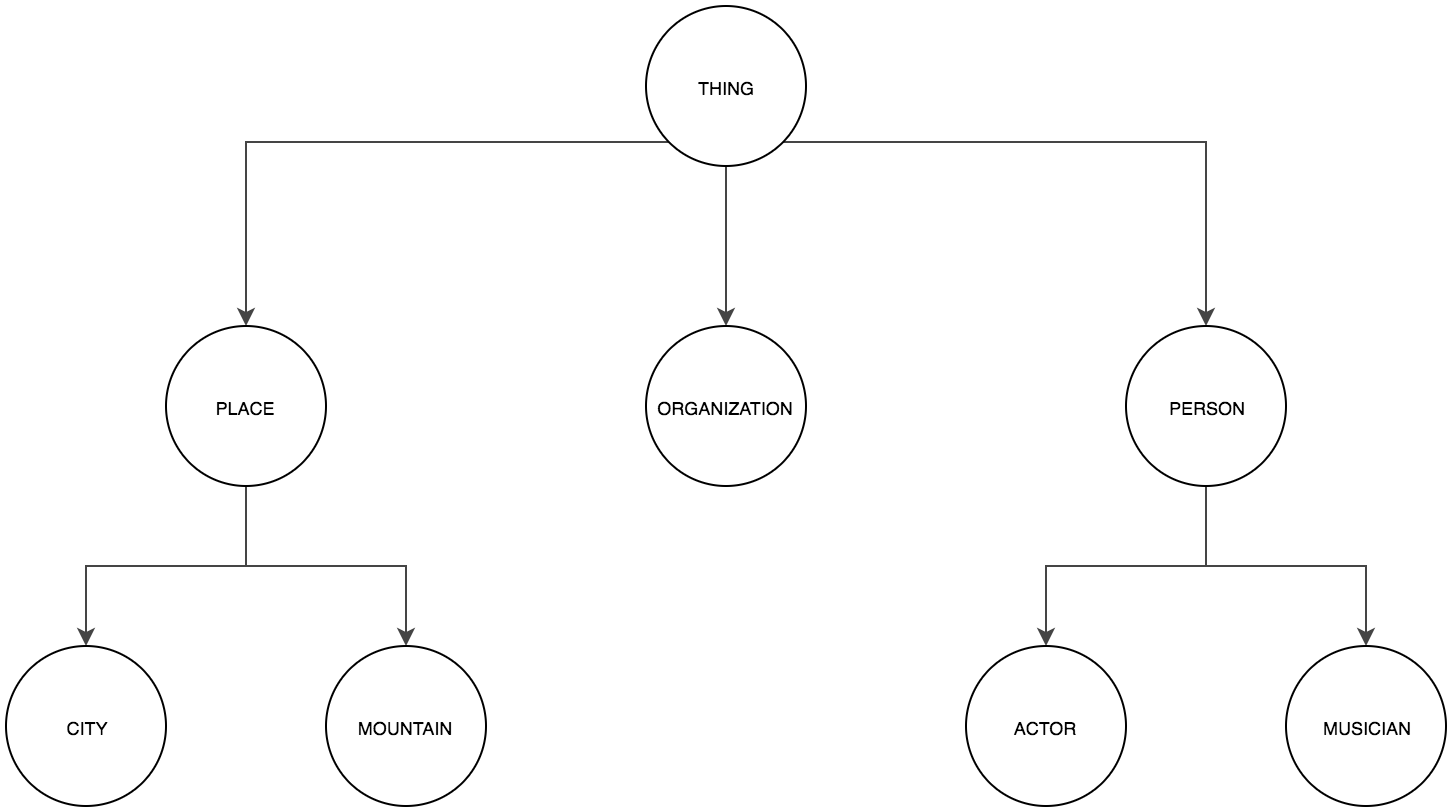
\includegraphics[scale=0.23]{onotlogy.png}
 	\caption{Example of type taxonomy for a generic extractor.}
 	\label{fig:ontology}
\end{figure}

We name $C_i$ the number of different types inside the level $i$ (e.g. $C_1 = 3$). We infer a one-hot encoding representation for each level as shown in \tabref{tab:onehottype}.

\begin{table}
\centering
\label{tab:onehottype}
\begin{tabular}{|c|c|c|c|}
\hline
\multicolumn{2}{|c|}{\textbf{LEVEL 1}} & \multicolumn{2}{|c|}{\textbf{LEVEL 2}} \\ \hline
\textbf{Type}  & \textbf{Representation}  & \textbf{Type}  & \textbf{Representation}    \\ \hline
PERSON          & 001   & ACTOR     & 0001  \\ \hline
ORGANIZATION    & 010   & MUSICIAN  & 0010  \\ \hline
PLACE           & 100   & CITY      & 0100  \\ \hline
      &       & MOUNTAIN  & 1000  \\ \hline
\end{tabular}
\bigskip
\caption{Representation of types through one-hot encoding.}
\end{table}

For a generic type $\tau$ in the last layer (e.g. ACTOR), the features vector $v_{\tau}$ consists in the concatenation of the one-hot representation of each type founded on the walk from the root to the leaf associate to $\tau$. The features vector for ACTOR is therefore  \texttt{0010001}, where the first three values \texttt{001} derive from PERSON and the last four values \texttt{0001} derive from ACTOR. Hence, we can state that $dim(v_{\tau})= \sum_{i}^{L}C_i$. If the extractor $e \in T$ returns a type that is not the last level in the hierarchy, as PERSON, we fill the missing vector positions with \texttt{0}. The features vector $v_{PERSON}$ associated to PERSON is thus \texttt{0010000}. This mechanism is extensible to any taxonomy. However the $dim(v_{\tau})$ is different for each extractor, depending on the taxonomy that it uses. 

This procedure can be extended also to extractors that do not perform NER. A generic extractor $e$, where $e \in U \wedge e \not\in T$, returns a link for each entity. Following the interlinks between KBs, we can always obtain an entity in Wikidata. The type of the entity would be the class of this entity in Wikidata, which is the value of the property \textit{instance of (P31)}.\footnote{\label{P31} \url{https://www.wikidata.org/wiki/Property:P31}}. Those types are also represented through one-hot encoding.

For a \textbf{typed named entity} $w^t$ with the format \texttt{(surface form, type)}, the type feature vector $\vec{t^{w^{t}}_{e}}$ is computed for the extractor $e$ where $e \in U \lor e \in T$. $dim(\vec{t^{w^{t}}_{e}})$ varies accordingly to the considered extractor. In fact, we get a real-value numerical type representation without a type alignment phase. For this reason, the number of dimensions that forms the type features vector depends on the the number of types in the extractor taxonomy.

\textbf{Entity features}. These features represent the similarity between two Wikidata entities $w_1$ and $w_2$, as a vector of 5 dimensions. The first four dimensions correspond to \textbf{semantic knowledge}:
\begin{enumerate}
\begin{item}
the first dimension indicates if the compared entities share the same URI with a boolean. We can express this value as $S_{uri}(w_1,w_2)$; \end{item}
\begin{item}
the second dimension provides the string similarity between the labels $l_{w_1}$ and $l_{w_2}$ associated to the compared entities: 
$$S_{Lev}(w_1,w_2) = max(1-d_{Lev}(l_{w_1},l_{w_2})/\beta,0), \beta = 8$$

where $d_{Lev}(l_{w_1},l_{w_2})$ is the \textbf{Levenshtein distance} between the compared strings and $\beta$ is a constant equals to the number of maximum differences after which the similarity is saturated to 0.
\end{item}
\begin{item}
the third dimension represents the \textbf{TF-IDF Cosine Similarity} between the abstracts associated to the compared entities. We can express this value as $S_{TfIdf}(w_1,w_2)$. This dimension represents a textual knowledge as in~\cite{CollaborativeKnowledgeBaseEmbeddingforRecommenderSystems};
\end{item}
\begin{item}
the fourth dimension value indicates if the compared entities share the same \textit{occupation (P106)}.\footnote{\url{https://www.wikidata.org/wiki/Property:P106}} We can express this value as $S_{occ}(w_1,w_2)$. This property is specific for entities of type PERSON: this wikidata class has no other subclasses, contrary to the other types. For this reason this similarity dimension greatly helps in the disambiguation of people with similar names but different professions.  $S_{occ}(w_1,w_2)$ is set to 1 when the two entities referred to people that have the same profession, and 0 otherwise.
\end{item}
\end{enumerate}

The fifth and last dimension of the vector represents the structural similarity as in~\cite{CollaborativeKnowledgeBaseEmbeddingforRecommenderSystems}. We define a property set $P$, containing three properties:
\textit{subclass of (P279)}\footnote{\url{https://www.wikidata.org/wiki/Property:P279}},
\textit{instance of (P31)}\footnote{\url{https://www.wikidata.org/wiki/Property:P31}}, and \textit{part of (P361)}.\footnote{\url{https://www.wikidata.org/wiki/Property:P361}}
A subgraph $G$ is realised by extracting from Wikidata all the triples in which a property in $P$ appears. We define the distance $d_{w_1,w_2}$ between two generic entities $w_1$ and $w_2$ as the shortest path length that links $w_1$ and $w_2$ in $G$. Then, we compute the maximum distance between two nodes in the graph $G$, defining it as $d_{max}$. We assess the structural similarity between $w_1$ and $w_2$ as:

$$S_{stc}(w_1,w_2) = -\frac{d_{w_1,w_2}}{d_{max}} + 1 $$

The total similarity between $w_1$ and $w_2$ can be expressed as:
\begin{equation}
\begin{gathered}
 \vec{S(w_1,w_2)} = \\
 = [S_{uri}(w_1,w_2),S_{Lev}(w_1,w_2),S_{TfIdf}(w_1,w_2),S_{occ}(w_1,w_2),S_{stc}(w_1,w_2)]
\end{gathered}
\end{equation}

The idea of representing the similarity between two entities as a real-value vectors rather than using an entity embedding arises from the fact that, in a ensemble perspective, our goal consists more in representing how the extractors differ in the named entities prediction than in directly representing an entity. Moreover, this approach avoids to compute embeddings on the whole Wikidata KB. We rely on interlinks between KBs for guaranteeing that we can always have Wikidata entities to compare with, even though some extractors provide disambiguation to other knowledge bases only. This causes the risk that no Wikidata entity exists for the source one, i.e. because the information is not present. However, this case is very rare (\tabref{tab:qmatch}) in all benchmarks we have evaluated our approach: the fact that all the involved extractors relies on Wikidata, Wikipedia or DBpedia -- containing similar information -- helps a lot for the mutual coverage of these knowledge bases. This would become a constraint when using different KBs (e.g. thematic ones), not fully interlinkable to Wikidata and for which it should take in consideration a loss in information.

\begin{table}
\centering
\label{tab:qmatch}
\begin{tabular}{|c|c|c|}
\hline
\textbf{Extractor} & \textbf{Disambiguation KB} & \textbf{WD Coverage} \\ \hline
Dandelion    & Wikipedia   & 99\%     \\ \hline
DBSpotlight  & DBpedia Fr  & 98\%     \\ \hline
TextRazor    & Wikidata    & 100\%    \\ \hline
Babelfy      & DBpedia     & 100\%    \\ \hline
\end{tabular}
\bigskip
\caption{Coverage of matching against Wikipedia of disambiguated entity in the ground truth.}
\end{table}

\textbf{Score features}. Some extractors return scores representing either the confidence or the saliency for each named entity. For each extractor $e \in K$, $w^k$ is a \textbf{score named entity} with the format \texttt{(surface form, scores)}. 
We define $\vec{k^{w^{k}}_{e}}$ as the the features vector representing the scores for the \textbf{score named entity} $w^k$ and the extractor $e$ where $e \in K$.  $dim(\vec{k^{w^{k}}_{e}})$ depends on the considered extractors, and more precisely, on the number of scores returned by a specific extractor.

%%%%%%%%%%%%%%%%%%%%%%%%%%%%%%%%%%%%%%%%%%
%%%  4. Ensemble NERD: ENNTR and ENND  %%%
%%%%%%%%%%%%%%%%%%%%%%%%%%%%%%%%%%%%%%%%%%

\section{Ensemble NERD: ENNTR and ENND}
\label{sec:experiment}
Our experimental ensemble method relies on two Neural Networks that receive in input the features described in the previous Section. We respectively name them with the acronyms \textbf{Ensemble Neural Network for Type Recognition (ENNTR)} and \textbf{Ensemble Neural Network for Disambiguation (ENND)}. For both networks, the hyper parameter optimization was done using Grid Search.

\subsubsection{Ensemble Neural Network for Type Recognition.}
We consider a generic ground truth $GT$ formed by $N$ textual fragments (e.g. sentences), such that we can split each fragment in tokens. $X_i$ is the ordered list of tokens for fragment $i$. Concatenating the lists $X_i$, we get a list $X$, that is the ordered list of tokens for all corpus. We call $x$ a generic token in $X$. 

$o_{GT}$ is the taxonomy associated to $GT$ and $card(o_{GT})$ represents the number of different types presented in $o_{GT}$ (its cardinality). $GT$ associates a type in $o_{Gt}$ to each token $x$. We identify the neural network target as $Y_t$. The number of samples in $Y_t$ is equal to the total number of tokens: $dim(Y_t)=dim(X)$. The neural network goal is to assign the right type to each token and its architecture is represented in Figure~\ref{fig:architecture_type_recognition}. 

\begin{figure}
	\centering
    	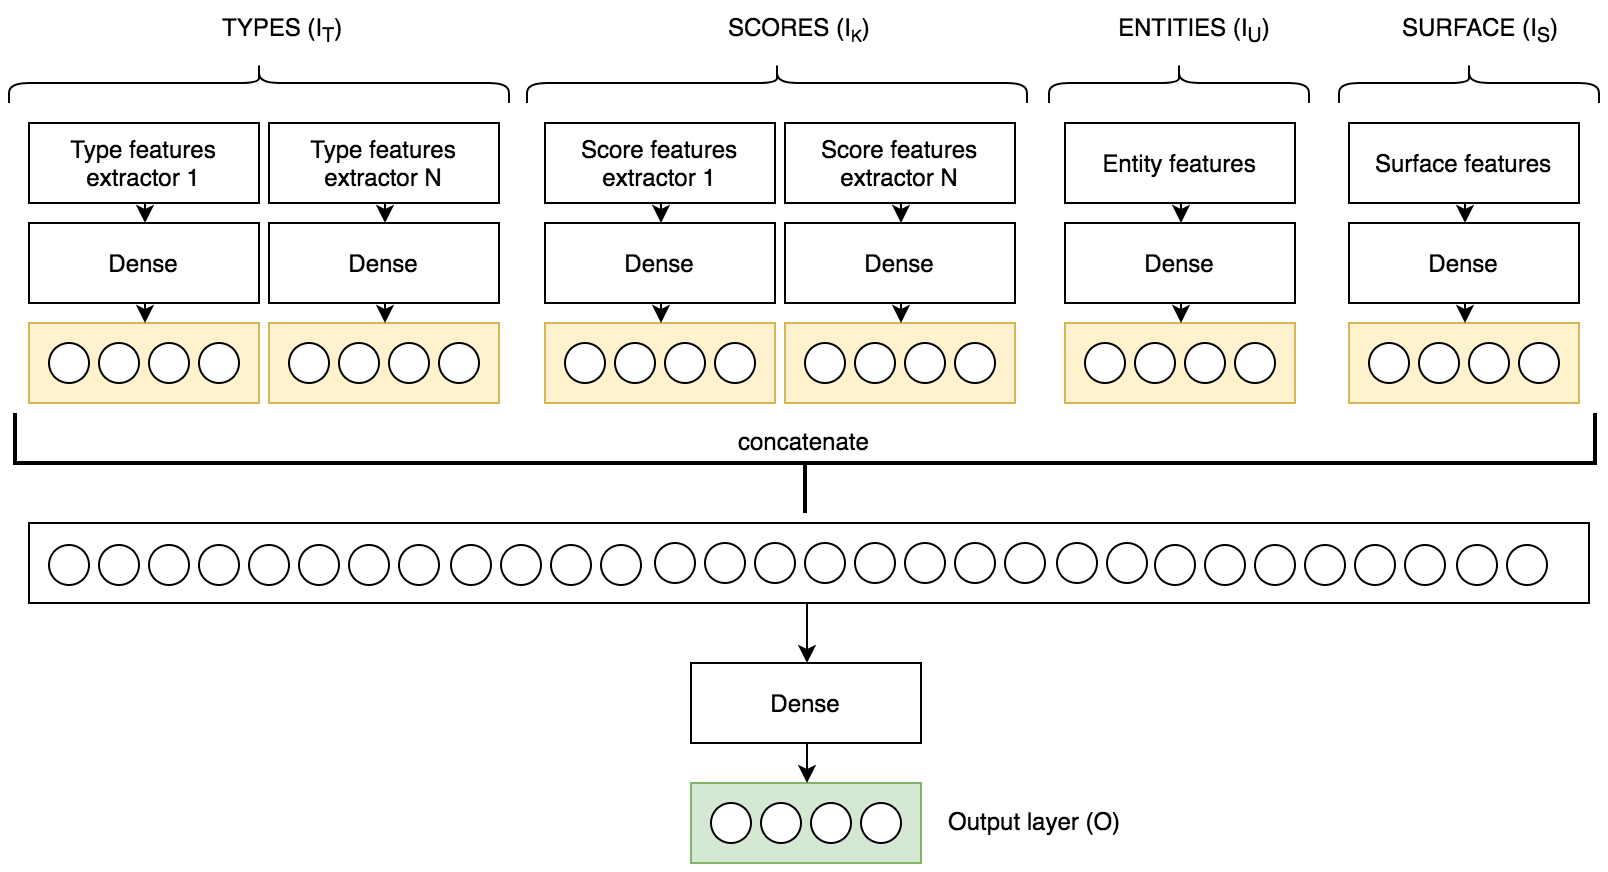
\includegraphics[scale=0.2]{architecture_type_recognition.png}
 	\caption{ENNTR architecture}
 	\label{fig:architecture_type_recognition}
\end{figure}

ENNTR has an output layer $O$ formed by $H$ neurons, such that $H=card(o_{GT})$. This means that the number of neurons in the output layer is equal to the number of types in the ground truth $GT$. For this reason, each value returned by a neuron in the output layer corresponds to the probability that a token $x$ is of a specific type. Hence, each target sample $\vec{y_t}$ is a vector formed by $H$ values, where each value corresponds to a type and a neuron. In Figure \ref{fig:architecture_type_recognition}, we are assuming that $H = 4$.

ENNTR presents many input layers. Using the same notation used in \secref{sec:study}, $T$ is the set of extractors that return type information, $K$ is the set of extractors that return score information, $U$ is the set of extractors that perform disambiguation. Defining $I$ as the set of input layers of ENNTR, we can identify four different types of input layer depending on the kind of features being input.

$$I = I_T \cup I_K \cup I_U \cup I_S$$
$$\left\vert{I}\right\vert= \left\vert{I_T}\right\vert + \left\vert{I_K}\right\vert + \left\vert{I_U}\right\vert + \left\vert{I_S}\right\vert  = \left\vert{T \cup U}\right\vert + \left\vert{K}\right\vert + 1 + 1$$

Each input sample that enters into $I_T$  is represented by a features vector $\vec{t^{x}_{e}}$, which is the features vector representing the type of the token $x$ for the extractor $e$ where $e \in U \lor e \in T$. In \secref{sec:study}, we defined $\vec{t^{w}_{e}}$ as the features vector representing the type for the named entity $w$ and the extractor $e$ where $e \in U \lor e \in T$. We focus on how to get $\vec{t^{x}_{e}}$ from $\vec{t^{w^{t}}_{e}}$. At each type named entity $w^{t}$ corresponds one or more tokens. Tokenizing $w^{t}$, we get a list of tokens $X_{w^{t}}$. Defining a default vector $\vec{d_t}$, such that $dim(\vec{d_t}) = dim(\vec{t^{w^{t}}_{e}})$  and containing only \texttt{0} values, we can get $\vec{t^{x}_{e}}$ as:

\begin{equation} \label{eq:type_feat}
\vec{t^{x}_{e}} = \left\{\begin{matrix} 
\vec{t^{w^{t}}_{e}} & if \: x \in X_{w^{t}}\\
\vec{d_t} & if \: x \notin X_{w^{t}}
\end{matrix}\right.
\end{equation}

Each input sample that enters into $I_K$  is represented by a features vector $\vec{k^{x}_{e}}$, which is the features vector representing the scores related to the token $x$ for the extractor $e$ where $e \in K$. Tokenizing $w^{k}$, we get a list of tokens $X_{w^{k}}$.
As for the type input layers, it is possible to derive $\vec{k^{x}_{e}}$ from $\vec{k^{w^{k}}_{e}}$:

\begin{equation} \label{eq:score_feat}
\vec{k^{x}_{e}} = \left\{\begin{matrix} 
\vec{k^{w^{k}}_{e}} & if \: x \in X_{w^{k}}\\
\vec{d_k} & if \: x \notin X_{w^{k}}
\end{matrix}\right.
\end{equation}

$$\vec{d_k} = [0,...,0], dim(d_k) == dim(\vec{k^{w^{k}}_{e}})$$

$w^u$ is a named entity with the format (surface form, link). Tokenizing $w^{u}$, we get a list of tokens $X_{w^{u}}$. $u^{w^{u}}_{e}$ is the Wikidata entity returned by the extractor $e$, where $e \in U$, for the entity $w^u$. $u^{x}_{e}$ is the Wikidata entity returned by the extractor $e$, where $e \in U$, for the token $x$. 

\begin{equation} \label{eq:score_feat}
u^{x}_{e} = \left\{\begin{matrix} 
u^{w^{u}}_{e} & if \: x \in X_{w^{u}}\\
NAN & if \: x \notin X_{w^{u}}
\end{matrix}\right.
\end{equation}

Considering that $card(U)=P$, we can now derive the entity features vector $\vec{u^{x}}$ for a token $x$ by applying the following equation: 

$$ \vec{u^{x}} = [S(u^{x}_{1},u^{x}_{1}),S(u^{x}_{1},u^{x}_{2}),...,S(u^{x}_{P},u^{x}_{P})] $$

The layers $I_U$ receive $\vec{u^{x}}$ as input. The input layers $I_S$ receive the surface features. A Fasttext features vector $\vec{s^{x}}$ corresponds to each token $x$. Each input layer $I_k$ is fully connected with a layer $M_k$. $M_k$, as $O$, is formed by $H$ neurons, where $H$ is the number of types in the ground truth. The activation of $M_k$ neurons is linear.

In this first part of the network, each $I_k$ (formed by a different number of neurons depending on the related features vector) is mapped on $H$ neurons in $M_k$. This avoids that the neural network privileges features vectors with higher dimension -- it happens directly concatenating different features vectors. This part of the network can be considered as an \textbf{alignment block} since it automatically map the types between the extractors and the ground truth taxonomy. This is pretty similar to the \textit{Inductive Entity Typing Alignment} work described in~\cite{nerd4}, with the difference that the alignment step is learned by a fully connected layer. Differently from previous works \cite{fox1,fox2}, the alignment and recognition phases are not anymore separated, because they are part of the same network. 

The last part of the network is the \textbf{ensemble block}. $M_k$ layers are concatenated forming a new layer $R$. $\left\vert{o_{GT}}\right\vert$ is the number of types in the ground truth, $\left\vert{I}\right\vert$ the number of input layers and $\left\vert{P}\right\vert$ the number of neurons in $R$:
 $$\left\vert{P}\right\vert =  \left\vert{o_{GT}}\right\vert \cdot \left\vert{I}\right\vert$$
 
$R$ is fully connected to the output layer $O$. The activation of the neurons in $O$ is linear. This means that ENNTR finally consists in a linear combinations of features: the key is the way in which the features are generated and entered in the network. The values $v_h$ of the $H$ output neurons in $O$ correspond to the probability that a given type is correct. We take the highest value $v_{max}$ between them and if it is greater than a threshold $\theta$, we set the type related to its neuron as the predicted one. The final output of the ensemble method is a list of predicted type $l_{p}$ for each token $x$. In a final step, sequences of token which belong to the same type are merged to a single entity, similarly to \cite{fox1,fox2}.

\subsubsection{Ensemble Neural Network for Disambiguation}
We consider a generic ground truth $GD$ formed by $N$ textual fragments, such that we can split each fragment in tokens. We express the number of tokens for a fragment $i$ as $M_i$. $X$ is the ordered list of tokens for all corpus, $x$ is a token in $X$. $GD$ associates a Wikidata entity identifier (URI) to each token. We identify the target as $Y_d$.

\begin{figure}[!ht]
	\centering
    	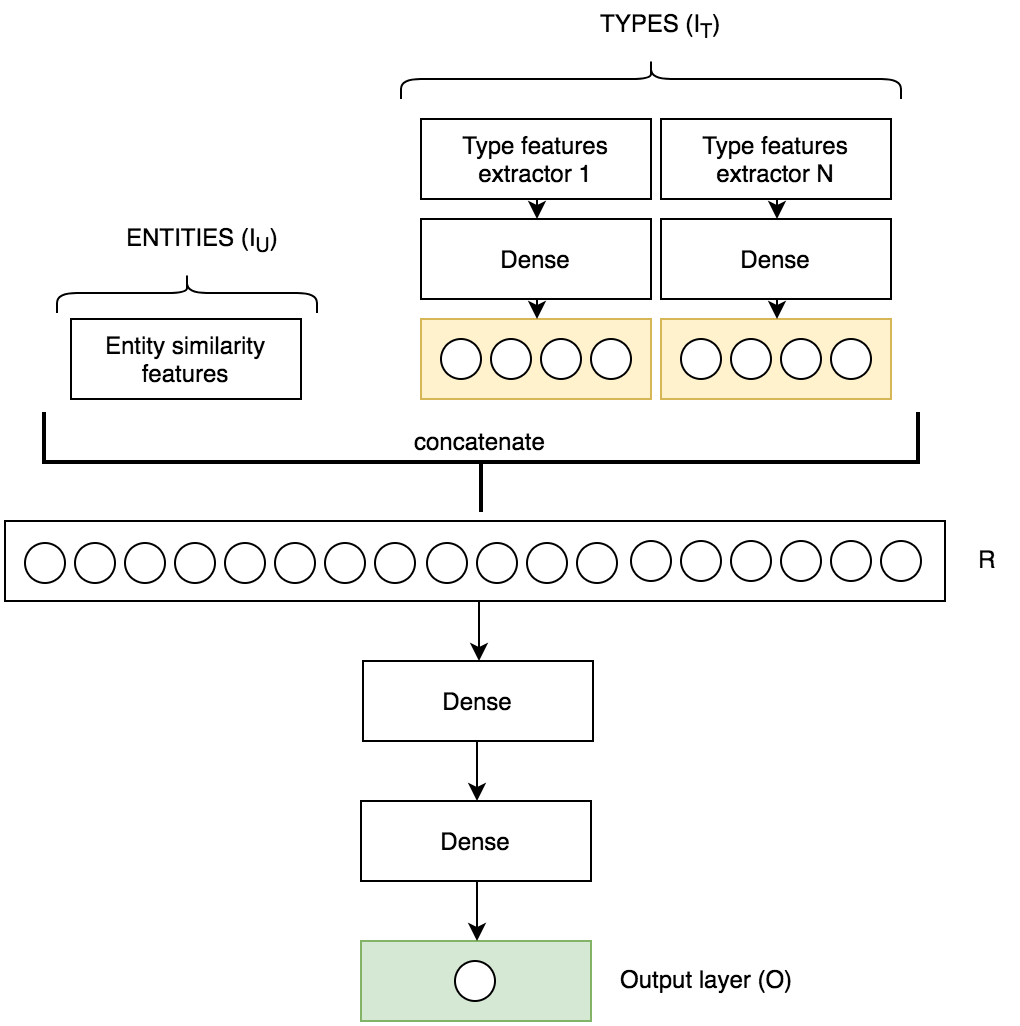
\includegraphics[scale=0.25]{NN_disambiguation.png}
 	\caption{ENND architecture}
 	\label{fig:NN_disambiguation}
\end{figure}

The ENND architecture is represented in \figref{fig:NN_disambiguation}. The goal of the network is to determine if the predicted entity by an extractor $e$, where $e \in U$, is correct, rather than to directly predict the right disambiguation Wikidata entity. For this reason, the number of samples in target $Y_d$ is not more equal to the number of tokens. For each token $x$, each extractor $e$ ($e \in U$) returns a predicted entity $\vec{u^{x}_{e}}$: we call $C_x$ the set of predicted entities for the token $x$, and  $v_x$ the correct entity; $\left\vert{C_x}\right\vert \leq \left\vert{U}\right\vert$ because more extractors could predict the same entity.
For each candidate $c_{x,j} \in C_x$, where $0 < j \leq \left\vert{C_x}\right\vert$, we generate a target sample $y_d \in Y_d$:
$$y_d  = \left\{\begin{matrix} 
1 & if \: c_{x,j} =  v_x\\
0 & if \: c_{x,j} \neq v_x
\end{matrix}\right.$$

The output layer $O$ contains a single neuron that should converge to $y_d$. The $O$ activation is a sigmoid. Naming $I$ the set of input layers of ENND, two different types of input can be identified depending on the kind of features.

$$I = I_U \cup I_T$$
$$\left\vert{I}\right\vert= \left\vert{I_U}\right\vert + \left\vert{I_T}\right\vert = 1 + \left\vert{T \cup U}\right\vert$$

The entity similarity features enter through $I_U$. We define $c_{x,j}$  as a candidate entity for the token $x$. For each target sample $y_d$, we compute a similarity features sample $\vec{u^{x,j}}$ as:

$$\vec{u_{x,j}} = [\vec{S}(c_{x,j},u^{x}_{1})|\vec{S}(c_{x,j},u^{x}_{2})|...|\vec{S}(c_{x,j},u^{x}_{R})] \: where \: R = card(U)$$
$$dim(\vec{u_{x,j}}) = dim(\vec{S(w_1,w_2)}) \cdot  card(U) $$

The input layers $I_T$ receives the features representing the type information. As for type recognition, for each $e \in U \lor e \in T$, the feature vector $\vec{t^{w^{t}}_{e}}$ represents the type for the named entity $w$, while $\vec{t^{x}_{e}}$ represents the type for the token $x$. $\vec{t^{x}_{e}}$ can be computed from $\vec{t^{w}_{e}}$ as described in \ref{eq:type_feat}. Considering that for each token $x$, there are multiple entity candidates, the vector $\vec{t^{w}_{e}}$ corresponding to the token $x$ is assigned to each candidate $p_{x,j}$, from which $p_{x,j}$ derives.

$I_T$ layers are fully connected to the layers $M_k$ as in ENNTR. $M_k$, as $O$, is formed by $H$ neurons. However, in this case, $H$ is no more the number of types in the ground truth, but it is an hyper-parameter. During our experiments, we set it to 4. As for ENNTR, the $M_k$ activation is linear.
 
After this step, the $I_U$ layer and the $M_k$ layers are concatenated in a new layer $R$. In this layer, some neurons represent the type information, some other the entity features. The idea is to exploit the fact that some extractors better disambiguate on certain types. The number of neurons in $R$ is equal to $dim(\vec{u_{x,j}}) + \left\vert{T \cup U}\right\vert \cdot H$.

The last part of the network is composed by two dense layers\footnote{A \textit{dense layer} is a layer fully connected to the previous one.} and the output layer $O$ discussed before. The activation functions of the dense layers are \textbf{Scaled Exponential Linear Units (selu)}:
$$selu(x) = \lambda \left\{\begin{matrix} 
x & if \: x > 0\\
\alpha e^{x} - \alpha & if \: x \leq 0 
\end{matrix}\right.$$

The loss function used to train the network is the Mean Square Error. The neural network goal is to determine the probability that an entity candidate is right. In fact, for each sample, we get an output value that corresponds to this probability.

$o_{x,j}$ corresponds to the output value of the input sample associated to the candidate entity $j$ for token $x$. Multiple candidates $C_x$ are associated to each token $x$. We select the candidate associated with the highest value $o_{x,max}$ among all output values $\left \{  o_{x,1},o_{x,2},...,o_{x,card(C_x)} \right \}$. Defining a threshold $\tau_d$, if $o_{x,max} > \tau_d$, we can select as predicted entity for token $x$ the one related to $o_{x,max}$. Otherwise, we connsider that the token $x$ is not part of a named entity. This process of \textbf{candidate selection} returns the list $z_{p}$ of predicted Wikidata entities identifiers at token level. In a final step, sequences of tokens which belong to the same Wikidata entity identifiers are merged to a single entity. $A_{p}$ represents the predicted corpus of annotated fragments as $A_{p}$.

%%%%%%%%%%%%%%%%%%%%%%%%%%%%%%%%%%%%%%
%%%  5. Experiment and Evaluation  %%%
%%%%%%%%%%%%%%%%%%%%%%%%%%%%%%%%%%%%%%

\section{Experiment and Evaluation}
\label{sec:evaluation}
We developed an implementation of the two neural networks using Keras.\footnote{The source code is available at \url{https://github.com/D2KLab/ensemble-nerd}, together with the documentation for accessing the live demo at \url{http://enerd.eurecom.fr}}
In order to make our approach comparable with the state of the art, our experiment evaluation relies on a well-known corpus and metrics, which have been already applied to related work. We alo evaluate our approach on another gold standard that we provide to the community.
\begin{itemize}
 \item \textbf{OKE2016}: annotated corpus of English textual resources, created for the 2016 OKE Challenge. The types set coincides with the one of OKE2015.
 \item \textbf{NexGenTv corpus}:\footnote{\url{http://enerd.eurecom.fr/data/training_data/nexgen_tv_corpus/}} this dataset is formed by 77 annotated fragments of transcripts from politician television debates in French.\footnote{The debates are in the context of the 2017 French presidential election.} Each fragment lasts in average 2 minutes. The corpus is split in 64 training and 13 test samples. The list of types includes 13 different labels.\footnote{PERSON, ORGANIZATION, GEOGRAPHICAL POINT, TIME, TIME INTERVAL, NUMBER, QUANTITY, OCCURRENCE, EVENT, INTELLECTUAL WORK, ROLE, GROUP OF HUMANS and OCCUPATION.} 
\end{itemize}

\subsubsection{Type recognition}
For each gold standard $GT$, two different kinds of score are computed.

The \textit{token based} scores have been used in \cite{fox1,fox2}. From $GT$, a list of target types $l_{t}$ with dimension $\left\vert{X}\right\vert$ is extracted. We can obtain from ENNTR the list of predicted types $l_{p}$. For each type $t_{GT}$ in $GT$, we compute precision $Precision(l_{t},l_{p},t_{GT})$, recall $Recall(l_{t},l_{p},t_{GT})$ and F1 score $F1(l_{t},l_{p},t_{GT})$. Then, we compute micro averaged measures $Precision_{micro}(l_{t},l_{p})$, $Recall_{micro}(l_{t},l_{p})$ and $F1_{micro}(l_{t},l_{p})$. \cite{sebastiani2002mltext}

The \textit{entity based} scores follow the definition of precision and recall coming from the \textbf{MUC-7 test scoring}~\cite{M98-1024}. Given $A_{t}$ and $A_{p}$ as the annotated fragment in $GT$, the computed measures are 
$Precision_{brat}(A_{t},A_{p})$, $Recall_{brat}(A_{t},A_{p})$ and 
$F1_{brat}(A_{t},A_{p})$. 

%\todo{results type per type do not fit here. Put them on the repo?}

The computed scores for OKE2016 and NexGenTv corpus are reported in \tabref{typescoresOKE2016} and \tabref{typescoresNEXGENTV}. The tables show also the same metrics applied to single extractors, after that their output types have been mapped to the ones of $GT$ through the alignment block of ENNTR. For both token and entity scores, the ensemble method outperforms the single extractors for all metrics.

\begin{table}
    \setlength{\tabcolsep}{12pt}
    \centering
    \begin{tabular}{c|c|c|c|c|c|c|}
      \multicolumn{1}{c}{ } &
      \multicolumn{3}{|c|}{TOKEN BASED} & 
      \multicolumn{3}{|c|}{ENTITY BASED} \\
       \multicolumn{1}{c|}{ } & \textbf{fsc} & \textbf{pre} & \textbf{rec}
       & \textbf{fsc} & \textbf{pre} & \textbf{rec} \\ \hline
        \textbf{adel}            & 0,87   & 0,88   & 0,87 & 0,84  & 0,85  & 0,83 \\ \hline
        \textbf{alchemy}         & 0,79   & 0,93   & 0,68 & 0,88  & 0,92  & 0,86 \\ \hline
        \textbf{babelfy}         & 0,66   & 0,88   & 0,7  & 0,74  & 0,79  & 0,7  \\ \hline
        \textbf{dandelion}       & 0,64   & 0,89   & 0,51 & 0,78  & 0,83  & 0,75 \\ \hline
        \textbf{dbspotlight}     & 0,59   & 0,75   & 0,49 & 0,6   & 0,77  & 0,52 \\ \hline
        \textbf{meaning cloud}   & 0,59   & 0,91   & 0,44 & 0,72  & 0,78  & 0,69 \\ \hline
        \textbf{opencalais}      & 0,56   & 0,97   & 0,39 & 0,69  & 0,71  & 0,68 \\ \hline
        \textbf{textrazor}       & 0,74   & 0,86   & 0,65 & 0,77  & 0,81  & 0,74 \\ \hline \hline
        \textbf{ensemble}        & \textbf{0,91}   & \textbf{0,91}   & \textbf{0,91}  & \textbf{0,94} & \textbf{0,95}  & \textbf{0,92} \\ \hline
       \textbf{ensemble ($I=I_T$)}        & \textbf{0,88}   & \textbf{0,91}   & \textbf{0,85}  & \textbf{0,88} & \textbf{0,92}  & \textbf{0,84} \\\hline
       \textbf{ensemble ($I=I_S$)}        & \textbf{0.50}   & \textbf{0,53}   & \textbf{0,47}  & \textbf{0.50} & \textbf{0,52}  & \textbf{0,48} \\\hline    
       \textbf{ensemble ($I=I_U$)}        & \textbf{0.44}   & \textbf{0,47}   & \textbf{0,41}  & \textbf{0.43} & \textbf{0,43}  & \textbf{0,43} \\\hline
       \textbf{ensemble ($I=I_K$)}        & \textbf{0,37}   & \textbf{0,40}   & \textbf{0,34}  & \textbf{0,38} & \textbf{0,40}  & \textbf{0,36} \\\hline    
    \end{tabular}
    \caption{OKE2016 corpus NER Evaluation}
    \label{typescoresOKE2016}
\end{table}

\begin{table}
      \centering
      \setlength{\tabcolsep}{12pt}
      \begin{tabular}{c|c|c|c|c|c|c|}
      \multicolumn{1}{c}{ } &
      \multicolumn{3}{|c|}{TOKEN BASED} & 
      \multicolumn{3}{|c|}{ENTITY BASED} \\
      & \textbf{fsc} &\textbf{pre} & \textbf{rec} 
      & \textbf{fsc} &\textbf{pre} & \textbf{rec} 
      \\ \hline
      \textbf{adel}           & 0,68  & 0,84  & 0,57 & 0,75  & 0,83  & 0,7  \\ \hline
      \textbf{alchemy}        & 0,80  & 0,83  & 0,77 & 0,87  & 0,97  & 0,81 \\ \hline
      \textbf{babelfy}        & 0,55  & 0,83  & 0,41 & 0,65  & 0,74  & 0,59 \\ \hline
      \textbf{dandelion}      & 0,26  & 0.69  & 0,16 & 0,51  & 0,69  & 0,42 \\ \hline
      \textbf{dbspotlight}    & 0,48  & 0,75  & 0,34 & 0,5   & 0,61  & 0,45 \\ \hline
      \textbf{meaning cloud}  & 0,82  & 0,88  & 0,77 & 0,8   & 0,87  & 0,76 \\ \hline
      \textbf{opencalais}     & 0,58  & 0,81  & 0,45 & 0,81  & 0,9   & 0,76 \\ \hline
      \textbf{textrazor}      & 0,81  & 0,89  & 0,74 & 0,75  & 0,8   & 0,72 \\ \hline \hline
      \textbf{ensemble}       & \textbf{0,94}  & \textbf{0.97}  & \textbf{0,91}  & \textbf{0,92} & \textbf{0,98}  & \textbf{0,87} \\ \hline
      \textbf{ensemble ($I=I_T$)}        & \textbf{0,87}   & \textbf{0,91}   & \textbf{0,83}  & \textbf{0,89} & \textbf{0,93}  & \textbf{0,85} \\ \hline
       \textbf{ensemble ($I=I_S$)}        & \textbf{0.54}   & \textbf{0,58}   & \textbf{0,50}  & \textbf{0.53} & \textbf{0,56}  & \textbf{0.50} \\\hline    
       \textbf{ensemble ($I=I_U$)}        & \textbf{0.47}   & \textbf{0,49}   & \textbf{0,45}  & \textbf{0.46} & \textbf{0,47}  & \textbf{0,45} \\\hline
       \textbf{ensemble ($I=I_K$)}        & \textbf{0,40}   & \textbf{0,42}   & \textbf{0,38}  & \textbf{0,39} & \textbf{0,40}  & \textbf{0,38} \\\hline    
      \end{tabular}
    \caption{NexGenTv corpus NER Evaluation}
    \label{typescoresNEXGENTV}

\end{table}



In order to identify the most influencing features in the obtained results, ENTTR has been sequentially adapted and retrained in order to receive in input only a specific kind of features, i.e. only $I_T$, $I_K$, $I_U$ or $I_S$. The tokens based scores for these new trained networks reveals that the type features \textit{$I_T$} are the only ones that, used alone as input, continue to make ENTRR outperforming single extractors. The other feature kinds, while having a lower impact, are still improving the final results when combined in the ensemble.

\subsubsection{Entity Linking}

We evaluate the entity linking for both OKE2016 and NexGenTv corpus using the GERBIL framework\footnote{GERBIL is a general Linked Data benchmarking that offers an easy-to-use web-based platform for the agile comparison of annotators using multiple datasets and uniform measuring approaches.} and in particular micro scores for the experiment type ``Disambiguate to Knowledge Base'' (D2KB). The computed scores are reported in \tabref{linkscores} and \tabref{linkscoresmacro}; the ensemble method outperforms again the single extractors that it integrates for all metrics.


\begin{table}
      \centering
      \setlength{\tabcolsep}{5pt}
        \begin{tabular}{c|c|c|c|c|c|c|c|c|c|}
          \multicolumn{1}{c}{ } &
          \multicolumn{3}{|c|}{OKE2016} & 
          \multicolumn{3}{|c|}{NEXGEN} &
          \multicolumn{3}{|c|}{AIDA}\\
           \multicolumn{1}{c|}{ } & \textbf{fsc} & \textbf{pre} & \textbf{rec}
           & \textbf{fsc} & \textbf{pre} & \textbf{rec} & \textbf{fsc} & \textbf{pre} & \textbf{rec} \\ \hline
            \textbf{babelfy}         & 0,54  & 0,64   & 0,47  & 0,51  & 0,51 & 0,51 & 0,66 & 0,70 & 0,62  \\ \hline
            \textbf{dandelion}       & 0,59   & 0,77   & 0,48 & 0,34  & 0,50  & 0,26 & 0,45   & 0,66   & 0,34\\ \hline
            \textbf{dbspotlight}     & 0,39   & 0,53   & 0,30 & 0,38   & 0,29  & 0,54 & 0,47	& 0,65 & 0,36 \\ \hline
            \textbf{textrazor}       & 0,53   & 0,78   & 0,40 & 0,61  & 0,55  & 0,69 & 0,62 & 0.57 & 0.53\\ \hline \hline
            \textbf{ensemble}        & \textbf{0,66}   & \textbf{0,88}   & \textbf{0,52}  & \textbf{0,69} & \textbf{0,70}  & \textbf{0,64} & \textbf{0,68}   & \textbf{0,79}   & \textbf{0,60} \\ \hline
            \textbf{ensemble ($I=I_U$)}        & \textbf{0,59}   & \textbf{0,80}   & \textbf{0,47}  & \textbf{0,59} & \textbf{0,60}  & \textbf{0,58} 
            & \textbf{0,55}   & \textbf{0,60}   & \textbf{0,50} \\ \hline
            \textbf{ensemble ($I=I_T$)}        & \textbf{0,41}   & \textbf{0,45}   & \textbf{0,38}  & \textbf{0,42} & \textbf{0,47}  & \textbf{0,38} 
            & \textbf{0,48}   & \textbf{0,52}   & \textbf{0,45} \\ \hline
        \end{tabular}
    \caption{GERBIL Micro scores on OKE2016,NexGenTV and AIDA/CoNLL corpus}
    \label{linkscores}
\end{table}



\begin{table}
      \centering
      \setlength{\tabcolsep}{5pt}
        \begin{tabular}{c|c|c|c|c|c|c|c|c|c|}
          \multicolumn{1}{c}{ } &
          \multicolumn{3}{|c|}{OKE2016} & 
          \multicolumn{3}{|c|}{NEXGEN} &
          \multicolumn{3}{|c|}{AIDA}\\
           \multicolumn{1}{c|}{ } & \textbf{fsc} & \textbf{pre} & \textbf{rec}
           & \textbf{fsc} & \textbf{pre} & \textbf{rec} & \textbf{fsc} & \textbf{pre} & \textbf{rec} \\ \hline
            \textbf{babelfy}         & 0,54  & 0,65   & 0,47  & 0,51  & 0,52 & 0,51 & 0,60  & 0,65 & 0,57 \\ \hline
            \textbf{dandelion}       & 0,59   & 0,76   & 0,49 & 0,35  & 0,50  & 0,27 & 0,43  & 0,52 & 0,37 \\ \hline
            \textbf{dbspotlight}     & 0,39   & 0,52   & 0,32 & 0,38   & 0,29  & 0,55  & 0,45  & 0,63 & 0,37\\ \hline
            \textbf{textrazor}       & 0,54   & 0,77   & 0,42 & 0,61  & 0,54  & 0,71 & 0,57  & 0,78 & 0,45\\ \hline \hline
            \textbf{ensemble}        & \textbf{0,65}   & \textbf{0,86}   & \textbf{0,53}  & \textbf{0,67} & \textbf{0,69}  & \textbf{0,64} & \textbf{0,68}   & \textbf{0,76}   & \textbf{0,61} \\ \hline
            \textbf{ensemble ($I=I_U$)}        & \textbf{0,59}   & \textbf{0,77}   & \textbf{0,48}  & \textbf{0,59} & \textbf{0,59}  & \textbf{0,59} & \textbf{0,55}   & \textbf{0,59}   & \textbf{0,51}\\ \hline
            \textbf{ensemble ($I=I_T$)}        & \textbf{0,42} & \textbf{0,44}  & \textbf{0,40}  & \textbf{0,41} & \textbf{0,42}  & \textbf{0,40} & \textbf{0,49}   & \textbf{0,51}   & \textbf{0,47}\\ \hline
        \end{tabular}
    \caption{GERBIL Macro scores on OKE2016,NexGenTV and AIDA/CoNLL corpus}
    \label{linkscoresmacroo}
\end{table}



\begin{table}
      \centering
      \setlength{\tabcolsep}{12pt}
        \begin{tabular}{c|c|c|c|c|c|c|}
          \multicolumn{1}{c}{ } &
          \multicolumn{3}{|c|}{Micro scores} & 
          \multicolumn{3}{|c|}{Macro scores} \\
           \multicolumn{1}{c|}{ } & \textbf{fsc} & \textbf{pre} & \textbf{rec}
           & \textbf{fsc} & \textbf{pre} & \textbf{rec} \\ \hline
            \textbf{agdistis}         & 0,50  & 0,50   & 0,50  &  0,52  & 0,52   & 0,52  \\ \hline
            \textbf{aida}         & 0,49  & 0,63   & 0,41  &   0,5  & 0,64   & 0,42   \\ \hline
            \textbf{dexter}         & 0,44  & 0,92   & 0,29  &   0,43  & 0,81   & 0,31   \\ \hline
            \textbf{fox}         & 0,48  & 0,77   & 0,35  & 0,47  & 0,69   & 0,37   \\ \hline
            \textbf{freme ner}         & 0,31  & 0,57   & 0,21  &   0,26  & 0,27   & 0,25   \\ \hline
            \textbf{kea}         & 0,64  & 0,67   & 0,61  &   0,63  & 0,66   & 0,61  \\ \hline
            \textbf{pboh}         & 0,69  & 0,69   & 0,69  &   0,69  & 0,69   & 0,69   \\ \hline \hline
            \textbf{ensemble}        & \textbf{0,66}   & \textbf{0,88}   & \textbf{0,52} & \textbf{0,65}   & \textbf{0,86}   & \textbf{0,53}  \\ \hline
        \end{tabular}
    \caption{GERBIL scores on OKE2016}
    \label{linkscoresgerbiloke2016}
\end{table}




 




 \begin{table}
      \centering
      \setlength{\tabcolsep}{12pt}
        \begin{tabular}{c|c|c|c|c|c|c|}
          \multicolumn{1}{c}{ } &
          \multicolumn{3}{|c|}{Micro scores} & 
          \multicolumn{3}{|c|}{Macro scores} \\
           \multicolumn{1}{c|}{ } & \textbf{fsc} & \textbf{pre} & \textbf{rec}
           & \textbf{fsc} & \textbf{pre} & \textbf{rec} \\ \hline
            \textbf{agdistis}         & 0,58  & 0,58   & 0,58  &  0,59  & 0,59   & 0,59  \\ \hline
            \textbf{aida}         & 0,00  & 0,00   & 0,00  &   0,00  & 0,00   & 0,00   \\ \hline
            \textbf{dexter}         & 0,51  & 0,76   & 0,38  &   0,47  & 0,75   & 0,36   \\ \hline
            \textbf{fox}         & 0,57  & 0,63   & 0,51  & 0,56  & 0,64   & 0,51   \\ \hline
            \textbf{freme ner}         & 0,38  & 0,62   & 0,27  &   0,29  & 0,30   & 0,27   \\ \hline
            \textbf{kea}          & 0,00  & 0,00   & 0,00  &   0,00  & 0,00   & 0,00  \\ \hline
            \textbf{pboh}         & 0,00  & 0,00   & 0,00  &   0,00  & 0,00   & 0,00   \\ \hline \hline
            \textbf{ensemble}        & \textbf{0,68}   & \textbf{0,79}   & \textbf{0,60} & \textbf{0,68}   & \textbf{0,76}   & \textbf{0,61}  \\ \hline
        \end{tabular}
    \caption{GERBIL scores on AIDA-CoNLL}
    \label{linkscoresgerbilaida}
\end{table}




%%% ADDED




For entity disambiguation, the most influential features are the entity ones \textit{$I_U$}. However, the impact of type features \textit{$I_T$} is still crucial because its absence makes really lower the improvement of the ensemble method with respect to a single extractor prediction.

%%%%%%%%%%%%%%%%%%%%%%%%%%%%%%%%%%%%%%%
%%%  6. Conclusion and Future Work  %%%
%%%%%%%%%%%%%%%%%%%%%%%%%%%%%%%%%%%%%%%

\section{Conclusion and Future Work}
\label{sec:conclusion}
In this paper, we presented two multilingual ensemble methods which combine the responses of web services (extractors) performing Named Entity Recognition and Disambiguation. The method relies on two Neural Networks that outperform the single extractors respectively in NER and NED tasks. Furthermore, the NER network allows to avoid the manually type alignment between the type ontologies of each extractor and the ground truth ontology. We demonstrated the importance of the features generation for the success of these ensemble methods. In terms of NER, the type features play most of the work in the ensemble. For the NED task, while entity features have the greater impact, only a combination with type features really improve the effectiveness of the ensemble method with respect to single extractor predictions.

As future work, we plan to enhance the input feature set with Part of Speech tags features that would be assigned to each token. We also aim
to vary the neural network architecture, and in particular, we are planning to replace the dense layer receiving the surface features with a BiLSTM, which would also take in consideration the context in which the tokens are sequentially appearing. Finally, all the neural networks models have been trained when all extractors APIs were reachable. However, it happens that some APIs can be out of service for some reasons (e.g. maintenance). In those cases, even if it would continue working, the results of our ensemble method may be influenced by those partially invalid inputs. A training that involves some samples which simulates the extractors failures would make the network models more robust to API failures.

%%%%%%%%%%%%%%%%%%%%%%%%%%
%%%  Acknowledgements  %%%
%%%%%%%%%%%%%%%%%%%%%%%%%%

\section*{Acknowledgements}
This work has been partially supported by the French National Research Agency (ANR) within the ASRAEL project (ANR-15-CE23-0018), the French Fonds Unique Interminist\'eriel (FUI) within the NexGen-TV project and the European  Union's Horizon 2020 research and innovation programme via the project MeMAD (GA 780069).

% ---- Bibliography ----
\bibliographystyle{abbrv}
\bibliography{references}

\end{document} 
